%% This is file `elsarticle-template-1-num.tex',
%%
%% Copyright 2009 Elsevier Ltd
%%
%% This file is part of the 'Elsarticle Bundle'.
%% ---------------------------------------------
%%
%% It may be distributed under the conditions of the LaTeX Project Public
%% License, either version 1.2 of this license or (at your option) any
%% later version.  The latest version of this license is in
%%    http://www.latex-project.org/lppl.txt
%% and version 1.2 or later is part of all distributions of LaTeX
%% version 1999/12/01 or later.
%%
%% The list of all files belonging to the 'Elsarticle Bundle' is
%% given in the file `manifest.txt'.
%%
%% Template article for Elsevier's document class `elsarticle'
%% with numbered style bibliographic references
%%
%% $Id: elsarticle-template-1-num.tex 149 2009-10-08 05:01:15Z rishi $
%% $URL: http://lenova.river-valley.com/svn/elsbst/trunk/elsarticle-template-1-num.tex $
%%
\documentclass[preprint,12pt]{elsarticle}

%% Use the option review to obtain double line spacing
%% \documentclass[preprint,review,12pt]{elsarticle}

%% Use the options 1p,twocolumn; 3p; 3p,twocolumn; 5p; or 5p,twocolumn
%% for a journal layout:
%% \documentclass[final,1p,times]{elsarticle}
%% \documentclass[final,1p,times,twocolumn]{elsarticle}
%% \documentclass[final,3p,times]{elsarticle}
%% \documentclass[final,3p,times,twocolumn]{elsarticle}
%% \documentclass[final,5p,times]{elsarticle}
%% \documentclass[final,5p,times,twocolumn]{elsarticle}

%% if you use PostScript figures in your article
%% use the graphics package for simple commands
%% \usepackage{graphics}
%% or use the graphicx package for more complicated commands
%% \usepackage{graphicx}
%% or use the epsfig package if you prefer to use the old commands
%% \usepackage{epsfig}

%% The amssymb package provides various useful mathematical symbols
\usepackage{amssymb}
%% The amsthm package provides extended theorem environments
\usepackage{amsthm}

%% The lineno packages adds line numbers. Start line numbering with
%% \begin{linenumbers}, end it with \end{linenumbers}. Or switch it on
%% for the whole article with \linenumbers after \end{frontmatter}.
\usepackage{lineno}

%% natbib.sty is loaded by default. However, natbib options can be
%% provided with \biboptions{...} command. Following options are
%% valid:

%%   round  -  round parentheses are used (default)
%%   square -  square brackets are used   [option]
%%   curly  -  curly braces are used      {option}
%%   angle  -  angle brackets are used    <option>
%%   semicolon  -  multiple citations separated by semi-colon
%%   colon  - same as semicolon, an earlier confusion
%%   comma  -  separated by comma
%%   numbers-  selects numerical citations
%%   super  -  numerical citations as superscripts
%%   sort   -  sorts multiple citations according to order in ref. list
%%   sort&compress   -  like sort, but also compresses numerical citations
%%   compress - compresses without sorting
%%
%% \biboptions{comma,round}

% \biboptions{}
\usepackage{lmodern}
\usepackage[english]{babel} 
\usepackage[T1]{fontenc}
\usepackage[utf8]{inputenc}
\usepackage{caption}
\usepackage{amsmath}
\usepackage[customcolors]{hf-tikz}
\usepackage{empheq, mathtools}
\usepackage{xcolor}
\usepackage{enumitem}
\usepackage{amsmath,amsfonts,amssymb}
\usepackage{listings}
\usepackage{graphicx}
\usepackage{subfig}
\usepackage{algorithm}
\usepackage[noend]{algpseudocode}
\usepackage{pythonhighlight}
\usepackage{slashbox}

\definecolor{deepblue}{rgb}{0,0,0.5}
\definecolor{deepred}{rgb}{0.6,0,0}
\definecolor{deepgreen}{rgb}{0,0.5,0}


%\journal{Journal Name}

\begin{document}

\begin{frontmatter}

%% Title, authors and addresses

%% use the tnoteref command within \title for footnotes;
%% use the tnotetext command for the associated footnote;
%% use the fnref command within \author or \address for footnotes;
%% use the fntext command for the associated footnote;
%% use the corref command within \author for corresponding author footnotes;
%% use the cortext command for the associated footnote;
%% use the ead command for the email address,
%% and the form \ead[url] for the home page:
%%
%% \title{Title\tnoteref{label1}}
%% \tnotetext[label1]{}
%% \author{Name\corref{cor1}\fnref{label2}}
%% \ead{email address}
%% \ead[url]{home page}
%% \fntext[label2]{}
%% \cortext[cor1]{}
%% \address{Address\fnref{label3}}
%% \fntext[label3]{}

\title{Bayesian Approach to Extreme Value Theory:                                 
\hspace{40pt} \large{\textit{How to study unusual weather events?}}}

%% use optional labels to link authors explicitly to addresses:
%% \author[label1,label2]{<author name>}
%% \address[label1]{<address>}
%% \address[label2]{<address>}

\author{Davide Fabbrucci}
\author{Matteo Pierdomenico}
\author{Giacomo Randazzo} 
%\author{\\ Supervisors: Andrea Manzoni, Stefano Pagani}

%\address{Milano, Italia}

\begin{abstract}
 

\end{abstract}

\begin{keyword}
\end{keyword}

\end{frontmatter}

% \linenumbers


%%%%%%%%%%%%%%%%%%%%%%%% ARTICOLO %%%%%%%%%%%%%%%%%%%%%%%%

\section{Introduction}
\label{S:1}
\subsection{\textit{Extreme Value Theory}}
Due to their rarity, events like epidemies, high atmospheric pollutions or natural disasters have long captured the public's attention and often they are shrouded in mystery.\\
A particular branch of statistics, Extreme Value Theory (\textit{EVT}), offers insights to their inherent scarcity and stark magnitude. \\
Moreover, in the few last decades, the \textit{EVT} literature has grown considerably, with applied interest in engineering, oceanography, environment and economics, among others, and that is because it allows us extrapolate informations beyond the range of available data.
\\
Unlike other statistical approaches, which are more concerned with the 'center' of probability distributions, Extreme Value Theory focuses on the tails of the distributions, i.e. either on maxima or minimal values, the extreme deviations from the median.


\subsection{\textit{Approaches for practical extreme value analysis }}
Given an ordered sample of a given random variable (or Given a set of continuous observations?), there exist two approaches to select the extremes for the analysis.
\\ 
The first approach is called \textit{Block Maxima} approach and it relies in dividing the dataset into blocks sufficiently large and then, picking the maximum over each sample, deriving the block maxima series.
\\
The second approach is called \textit{Peak Over Threshold (POT)} and it consists in picking a threshold and extracting, from a continuous record, all the observation exceeding that threshold.

\subsection{\textit{Extreme daily high gust in Ireland (or The Dataset)}}

In this paper we use a Bayesian approach to develop models  for daily highest wind gusts over a region
of central and southern Ireland. The data that are used consists of daily maximum wind gusts recorded by the Irish National Meteorological Service at 5 locations (Fig \ref{figure:Ireland}), namely we considered 5 different counties (\textit{Clare, Clarke, Dublin, Kerry} and \textit{Westmeath}) and data recorded from one station for each county. 
For all the sites, data are recorded over a period of 30 years, from December 1st, 1990 to November 30th, 2020, constituting 54790 observations at each site.

\begin{figure}[!h]
\captionsetup[subfigure]{labelformat=empty}
\subfloat[]{\includegraphics[width=1.4\linewidth]{Immagini/Ireland}} \quad
\caption{Map of the wind speed stations considered with the relative 30 years daily time series of maximum daily wind gust.}
\label{figure:Ireland}
\end{figure}


In Fig. \ref{figure:Data} is illustrated an exploratory analysis of data from two contrasting sites, Kerry and Westmeath. The first is one of the  most mountainous regions of Ireland, it is bounded on the west by the Atlantic Ocean and it is more often exposed to intense atmospheric phenomena; the second is a county in the center of Ireland, the torritory is mostly constituted by hills and lakes and it has not boundaries with the sea.
The effects of these differences are clearly seen in Fig \ref{figure:Data}, where a time series plot, a plot of the time series against the lagged series and an histogram of the observations is represented for both the counties.

\begin{figure}[!h]
\captionsetup[subfigure]{labelformat=empty}
\subfloat[]{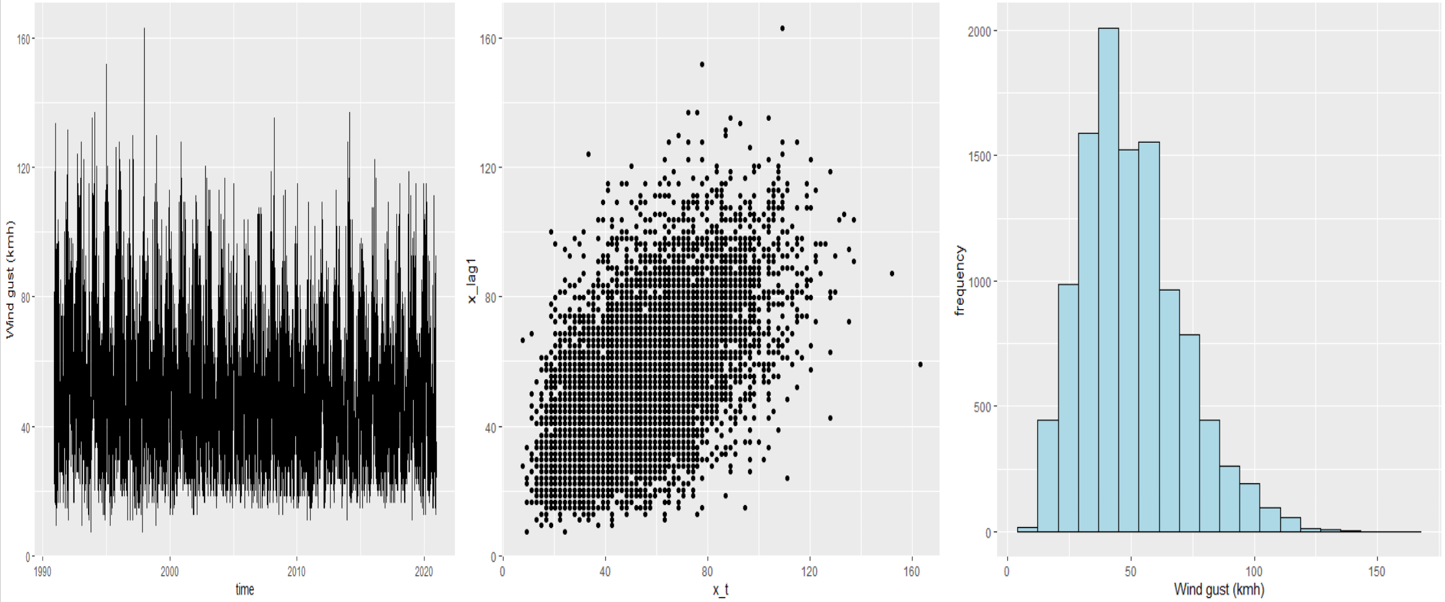
\includegraphics[width=1\linewidth]{Immagini/Kerry_data}} \quad
\subfloat[]{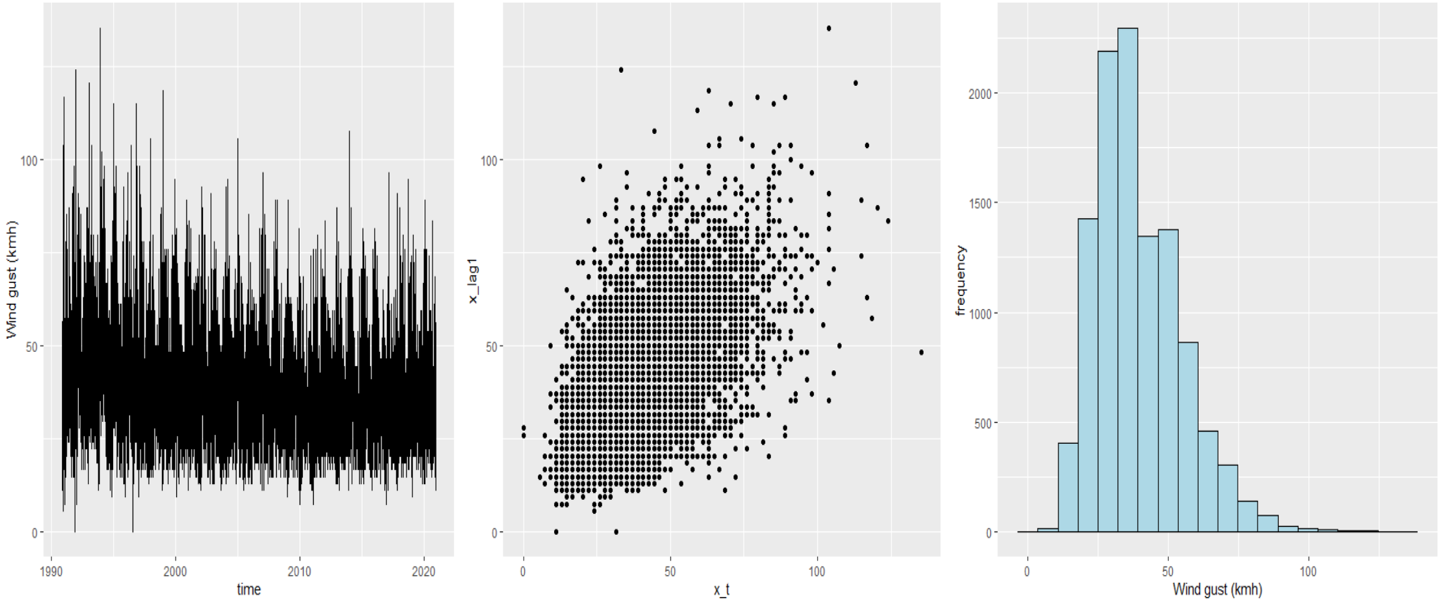
\includegraphics[width=1\linewidth]{Immagini/Westmeath_data}} \quad
\caption{Time series plot, plot of the time series against the lagged series and histograms of daily maximum wind gusts in Kerry (above) and Westmeath (below).}
\label{figure:Data}
\end{figure}

\subsection{\textit{The models}}



\section{Block Maxima Approach Model}
\section{POT Model}
\section{Hierarchical random effects model}
\section{Conclusions}

%%%%%%%%%%%%%%%%%%%%% BIBLIOGRAPHY %%%%%%%%%%%%%%%%%%%%%%%%%%
\clearpage
\begin{thebibliography}{99}
\end{thebibliography}
\end{document}



